\documentclass{standalone}
\usepackage{tikz}
\usepackage{ctex,siunitx,bm}
\setCJKmainfont{Noto Serif CJK SC}
\usepackage{tkz-euclide,ninecolors}
\usepackage{amsmath}
\usetikzlibrary{patterns, calc}
\usetikzlibrary {decorations.pathmorphing, decorations.pathreplacing, decorations.shapes,}
\begin{document}
\small
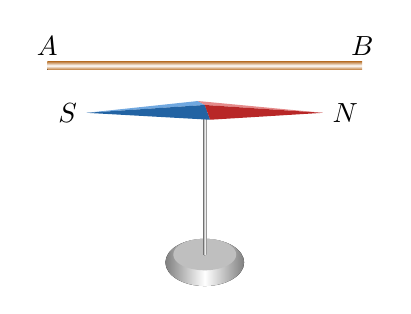
\begin{tikzpicture}[>=latex,yscale=1.0]
  \fill[left color=gray,right color=gray,middle color=white](0,0)ellipse(0.5 and 0.3);
  \fill[lightgray](0,0.1)ellipse(0.4 and 0.2);
  \fill[left color=gray,right color=gray,middle color=white](0,0.1)ellipse(0.02 and 0.01);
  \fill[left color=gray,right color=gray,middle color=white](-0.02,0.1)rectangle(0.02,2.0);
  \fill[azure7](0,2.0)--++(150:0.1)--(-1.5,1.9)node[text=black,left]{$S$};
  \fill[azure4](0,2.0)--++(290:0.2)--(-1.5,1.9);
  \fill[red7](0,2.0)--++(150:0.1)--(1.5,1.9)node[text=black,right]{$N$};
  \fill[red4](0,2.0)--++(290:0.2)--(1.5,1.9);
  \fill[top color=brown,bottom color=brown,middle color=white](-2,2.45)rectangle(2,2.55);
  \node at (-2,2.5)[above]{$A$};
  \node at (2,2.5)[above]{$B$};
\end{tikzpicture}
\end{document}